With the advent of multicore processors,there has been a renewed interest in the development of performance tools and algorithms targeted for parallel architectures. Many research areas  provide a wide variety of problems which would show improved performance when executed in parallel. One such area is scientific and numerical computing. Scientic algorithms are used by researchers from various fields such as chemistry, biology, geography etc. as well as different sub-fields of computer science like machine learning. In most cases, these algorithms are written in languages  that are collectively known as  array based languages. A few examples of such languages are \matlab\cite{matlab}, Julia\cite{julia} and Python\cite{python} with it's NumPy\cite{numpy} library.\\
Array based languages offer features like, a interpreter style read-eval-print-eval,functions such as eval and feval for dynamic code evaluation,  no types etc. which enable rapid prototyping. However due to the very same features, these languages show poorer performance when compared to statically compiled languages. A common approach for improving the performance is compile whole programs to languages such as {\sc FORTRAN} and C. However, in most cases, the most computationally intensive portion of the program is small, often localised inside a loop body. Hence compiling the entire program is not necessary. In most cases speed up observed through partial compilation of hot code sections is commensurate with that observed by compiling the whole program. This allows the user to continue programming in the language he/she is more comfortable in.\\
This thesis addresses the problem of improving the performance of programs written in array based languages by compiling the hot sections to parallel C++. We support both \matlab\cite{matlab} and Numpy\cite{numpy}. There are two main challenges. First one is supporting the different and often complementary semantics of both languages. The other is supporting the large number of builtins methods that are supported by both languages.
Our solution implement a static C++ backend for Velociraptor\cite{velociraptor} toolkit and use tools to compile matlab\cite{matlab} and Python\cite{python} programs to the Velociraptor\cite{velociraptor} intermediate representation, VRIR. The McLab static pipeline is used for \matlab\cite{matlab} and PyVrir, a Python\cite{python} frontend for Velociraptor\cite{velociraptor} is used for Python\cite{python}. 
\section{\velocty compilation pipeline}
The compilation pipeline for \velocty can be seen in \ref{Fig:Overview}. As mentioned earlier, PyVrir is a proof of concept Python\cite{python} frontend that is part of the Velociraptor\cite{velociraptor} framework and the \matlab\cite{matlab} frontend is written using the \mclab frontend. In the \mclab pipeline a \matlab\cite{matlab} program is parsed by the \mclab frontend and converted into an AST based representation known as McAST. The McSAF\cite{doherty11} framework then performs various analyses such as kind analyses and function lookup on McAST and then generates another AST based representation called McLAST. The framework also performs a colon2range transformation that was implemented as part of this thesis. Additional details on the colon2range analysis can be found in \chapref{chap:McSAFTranslate}. McLAST is then converted to TameIR\cite{Dubrau:2012} by the Tamer\cite{Dubrau:2012} framework. TameIR\cite{Dubrau:2012} is a three address representation of \matlab\cite{matlab}. Analyses such as value analysis, shape analysis, isComplex analysis and IntegerOk analysis are performed on this IR. These analyses provide information on the type, dimensions and complexity of different variables code which is useful for generating the VRIR and subsequently the C++ code. The IntegerOk analysis identifies variables which can safely be declared as integers in the target language. This analysis is useful since \matlab\cite{matlab} defines all variables as double by default. TameIR\cite{Dubrau:2012} is then given as input to Tamer+, a code aggregation framework, which generates the high-level McLAST representation from it. Code generated from McLAST is devoid of temporary variables and hence has better readability.The VRIR code generator takes McLAST as input and generates VRIR in the s-expression format. It also generates, glue code using the \matlab\cite{matlab} Mex\cite{mex} API which is required for interfacing with \matlab\cite{matlab}.\\ 
The VRIR is then parsed by the Velociraptor\cite{velociraptor} frontend and converted into an AST representation. Various passes such as the simplification pass, loop info collector and the index info collector pass are performed over the AST and is then passed to the static code generator. Finally, the code generator outputs C++ code which can then be compiled to a shared library along with the language specific run time library containing helper functions and the glue code. 
\begin{figure}[htbp]
\begin{center}
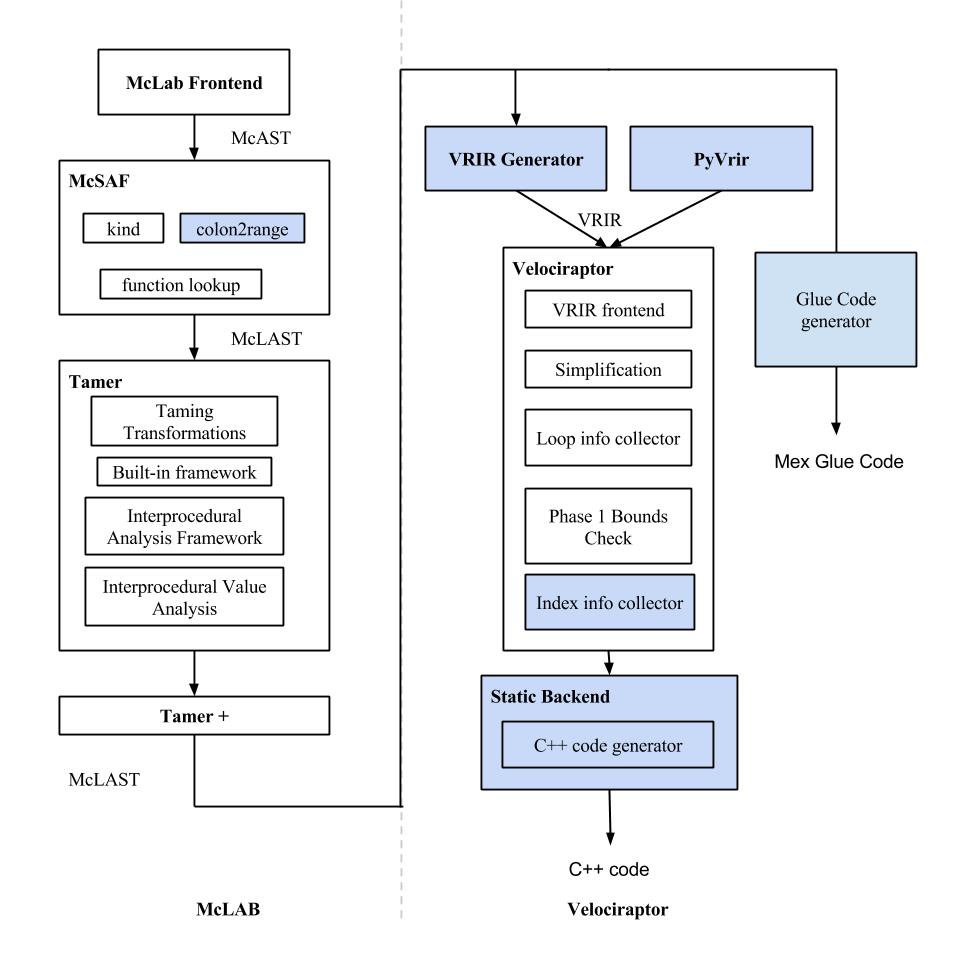
\includegraphics[scale=0.5]{Figures/Overview_thesis.png}
\caption[Overview of the VeloCty]{Overview
of VeloCty. The shaded boxes indicate the components
presented in this thesis. The other solid boxes correspond to
existing \mclab and Velociraptor\cite{velociraptor} tools we use}\label{Fig:Overview}
\end{center}
\end{figure}
\section{The Execution Model} 
The Execution model, shown in figure \ref{Fig:working}, describes how program execution occurs before and after statically compiling some of the methods in the program to C++ using \velocty. The user selects a function which he/she identifies as computationally intensive. \velocty generates a callgraph using the user-specified function as an entry point. In figure \ref{Fig:working} the coreFunction1 is specified as the entry point and the  generated callgraph contains coreFunction1 and coreFunction2. Both these functions are compiled by \velocty to C++.\\
The generated C++ code contains calls to functions in a language-specific library. The library contains functions which mirror the builtins in the source language. These functions are also written in C++ but are language-specific because the behaviour of the functions are dependent on the source language.\\
\velocty also generates glue code to interface with the source program. The Mex\cite{mex} API and the Python\cite{python} C API are used for interfacing with \matlab and Python\cite{python} respectively.\\
The generated code is compiled with the runtime and the glue code and packaged as a shared library. All calls to the entry point function, in this case, coreFunction1, would be directed to the shared library instead of the original source language version.\\
\begin{figure}[htbp]
\begin{center}
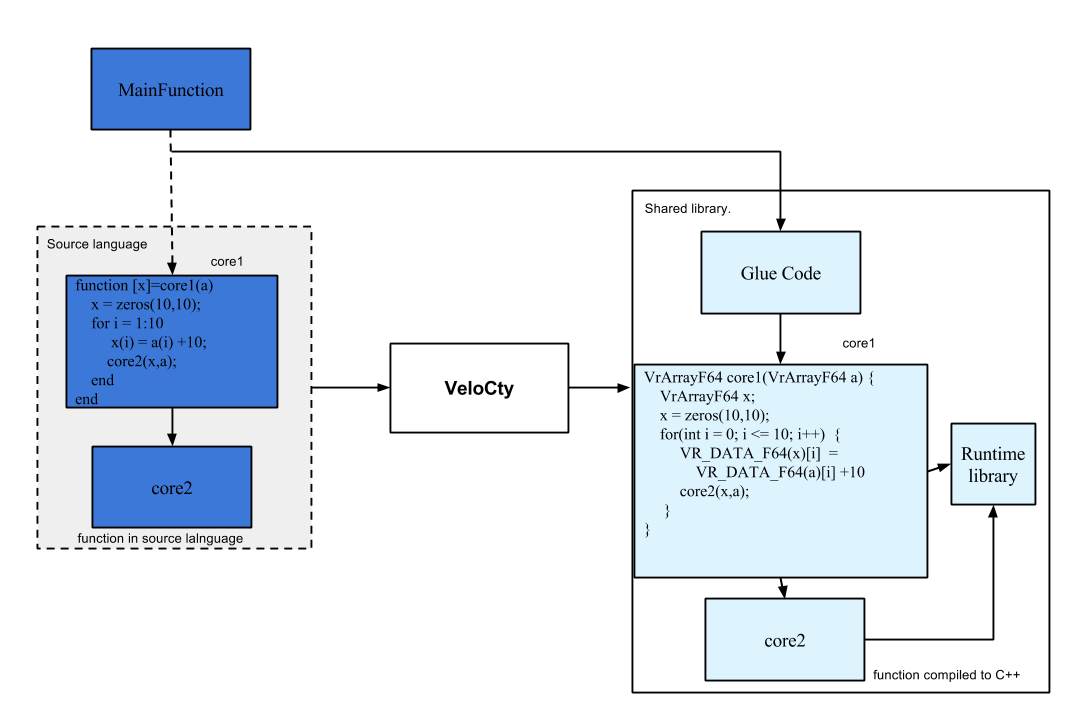
\includegraphics[scale=0.4]{Figures/WorkingDetails.png}
\caption[Execution Model]{Execution model of VeloCty. The dark shaded blocks represent functions written in the source language and the blocks that are lightly shaded are the functions written in C++. The white block represents the \velocty compiler.}\label{Fig:working}
\end{center}
\end{figure}
\section{Contributions}
The main contributions of this thesis are as follows.
\begin{itemize}
\item Generating the Velociraptor\cite{velociraptor} intermediate representation from the McSAF\cite{doherty11} intermediate representation. 
\item Implementation of a transformation from  Colon expressions to Range expressions
\item Generating glue code necessary for invoking C++ functions from \matlab\cite{matlab}.
\item Generating C++ code from the Velociraptor\cite{velociraptor} IR.
\item Optimizing generated code by elminating bounds checks and removing unncessary memory allocations. 
\end{itemize}
\section{Thesis Outline}
This thesis is divided into \ref{chap:Conclusions} chapters, including this one, which are structured as follows.
\chapref{chap:Background} gives a brief overview of the tools
used by VeloCty.
\chapref{chap:McSAFTranslate} describes the translation from the McSAF\cite{doherty11}.
intermediate representation to the Velociraptor\cite{velociraptor} intermediate representation(VRIR).
\chapref{chap:glueCode} describes the various aspects of generating glue code for \matlab\cite{matlab}'s Mex API including how input data is converted from Mex data structures to VeloCty data structures. 
\chapref{chap:vrirBackend} talks about the generation of C++ code from VRIR.
\chapref{chap:codeOptimise} explains the code optimisations implemented to improve the performance. 
\chapref{chap:Related} provides an overview of related work and
\chapref{chap:Conclusions} concludes.
